%%%%%%%%%%%%%%%%%%%%%%%%%%%%
% SECTION                  %
%%%%%%%%%%%%%%%%%%%%%%%%%%%%
\vspace{1em}

Les IDS, notamment ceux faisant de la détection par signatures, ont besoin d'une base de référentiels pour savoir quoi détecter. C'est ce rôle que jouent les indicateurs de compromission (ou IOC : Indicator Of Compromise)\\

Un indicateur de compromission, en sécurité informatique, est une déviance ou un artéfact observé sur un réseau ou dans un système d'exploitation qui indique, avec un niveau de certitude déterminé, une intrusion informatique. Des indicateurs de compromission peuvent être : des signatures virales, des adresses IP particulières, des hachages de fichiers malveillants, des URLs ou des noms de domaine de serveurs de commande et de contrôle de botnets, etc. \hyperref[biblio]{[4]}\\

\begin{figure}[h]%
    \center%
    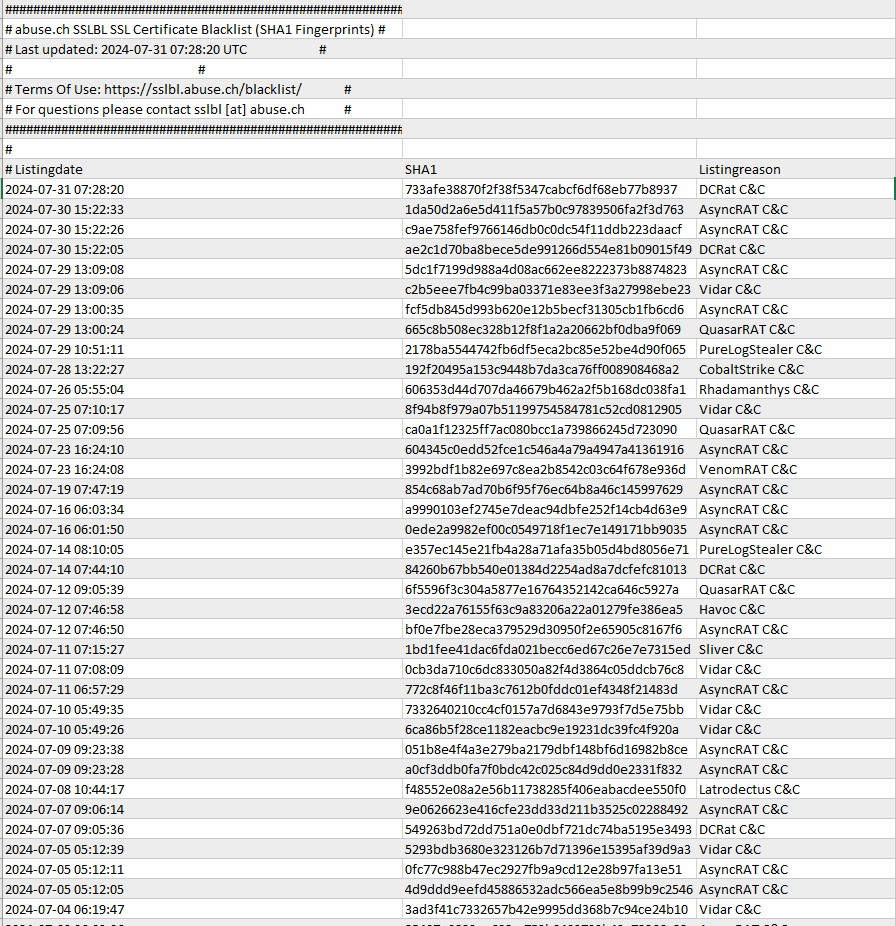
\includegraphics[width=0.74\textwidth]{assets/IOC.png}
    \caption[Exemple de liste d'IOC de hachages de fichiers malveillants fournie par \textit{abuse.ch} (source: \href{https://sslbl.abuse.ch/blacklist/sslblacklist.csv}{sslbl.abuse.ch/blacklist/sslblacklist.csv})]{Exemple de liste d'IOC de hachages de fichiers malveillants fournie par \textit{abuse.ch}}\label{fig:ioc}
\end{figure}

\newpage

Ces IOC sont découverts à la suite d'investigations numériques (également appelées renseignements sur les menaces ou \textit{threat intelligence}) menées sur les traces laissées par des acteurs malveillants en ligne ou à partir d'une analyse post-incident des techniques utilisées par les attaquants qui ont tenté ou réussi à pénétrer dans le système informatique. Ces IOC sont ensuite partagés par différents acteurs:\\

\begin{itemize}[itemsep=1em]
    \item[•] \textbf{Organismes de cybersécurité}\\
    La plupart des CERT étatiques (CERT-FR Français, US-CERT Américains, etc.) ou privés (CERT Orange, CERT Crédit Agricole, etc.) réalisent en partie eux-mêmes de la collecte d'IOC qu'ils partagent en privé entre agences lorsque des accords de collaboration existent, mais aussi publiquement pour une part\footnote{Exemple source publique du CERT-FR: \url{https://www.cert.ssi.gouv.fr/ioc/}}.
    \item[•] \textbf{Entreprises spécialisées de CTI}\\
    Le besoin de renseignement sur les menaces existantes ne cessant de croître, des sociétés spécialisées se sont créées pour répondre à cette demande (CrowdStrike, Sekoia.io, etc.) en plus des autres services de cybersécurité qu'elles peuvent pourvoir. En échange d'un contrat rémunéré, ces sociétés fournissent des listes d'IOC régulièrement mises à jour.
    \item[•] \textbf{Plate-formes d'échange libre de renseignement cyber}\\
    Pour faire face à l'ampleur des menaces, des plateformes de coopération CTI ont commencé à apparaître en ligne, impliquant des organisations étatiques et privées ainsi que des professionnels individuels du secteur. Grâce à ces plateformes (MISP, alienvault, threatfox, etc.), les utilisateurs peuvent s'alerter mutuellement des évènements cyber en cours et partager les IOC qu'ils possèdent.
\end{itemize}